\documentclass{beamer}

\mode<presentation> {

%\usetheme{default}
%\usetheme{AnnArbor}
%\usetheme{Antibes}
%\usetheme{Bergen}
%\usetheme{Berkeley}
%\usetheme{Berlin}
%\usetheme{Boadilla}
\usetheme{CambridgeUS}
%\usetheme{Copenhagen}
%\usetheme{Darmstadt}
%\usetheme{Dresden}
%\usetheme{Frankfurt}
%\usetheme{Goettingen}
%\usetheme{Hannover}
%\usetheme{Ilmenau}
%\usetheme{JuanLesPins}
%\usetheme{Luebeck}
%\usetheme{Madrid}
%\usetheme{Malmoe}
%\usetheme{Marburg}
%\usetheme{Montpellier}
%\usetheme{PaloAlto}
%\usetheme{Pittsburgh}
%\usetheme{Rochester}
%\usetheme{Singapore}
%\usetheme{Szeged}
%\usetheme{Warsaw}

% As well as themes, the Beamer class has a number of color themes
% for any slide theme. Uncomment each of these in turn to see how it
% changes the colors of your current slide theme.

%\usecolortheme{albatross}
%\usecolortheme{beaver}
%\usecolortheme{beetle}
%\usecolortheme{crane}
%\usecolortheme{dolphin}
%\usecolortheme{dove}
%\usecolortheme{fly}
%\usecolortheme{lily}
%\usecolortheme{orchid}
%\usecolortheme{rose}
%\usecolortheme{seagull}
%\usecolortheme{seahorse}
%\usecolortheme{whale}
%\usecolortheme{wolverine}

%\setbeamertemplate{footline} % To remove the footer line in all slides uncomment this line
%\setbeamertemplate{footline}[page number] % To replace the footer line in all slides with a simple slide count uncomment this line

%\setbeamertemplate{navigation symbols}{} % To remove the navigation symbols from the bottom of all slides uncomment this line
}

\usepackage{graphicx} % Allows including images
\usepackage{booktabs} % Allows the use of \toprule, \midrule and \bottomrule in tables
\usepackage{tikz}
\usetikzlibrary{shapes.geometric, arrows}
\tikzstyle{startstop} = [rectangle, rounded corners, minimum width=4cm, minimum height=1.3cm,text centered, draw=black, fill=red!30]
\tikzstyle{process} = [rectangle, minimum width=4cm, minimum height=1.3cm, text centered, draw=black, fill=orange!30]
\tikzstyle{decision} = [diamond, minimum width=4cm, minimum height=1.3cm, text centered, draw=black, fill=green!30]
\tikzstyle{arrow} = [thick,->,>=stealth]

\tikzstyle{dfdprocess} = [circle,draw=black, inner sep=0pt,minimum size=3cm, fill=red!30, text width=3cm, text centered]
\tikzstyle{dfdentity} = [rectangle, rounded corners, minimum width=3cm, minimum height=1.2cm,text centered, draw=black, fill=red!30]
\tikzset{data store/.style={
        minimum width=4.5cm,
        minimum height=1.2cm,
        append after command={
            \pgfextra
            \fill[fill=red!30] (\tikzlastnode.south east) [rounded corners] -| (\tikzlastnode.west) |- (\tikzlastnode.north) [sharp corners] -| (\tikzlastnode.north east)--cycle;
            \draw[rounded corners] (\tikzlastnode.south east) -| (\tikzlastnode.west) |- (\tikzlastnode.north east);
        \endpgfextra}
    }
}
%----------------------------------------------------------------------------------------
%	TITLE PAGE
%----------------------------------------------------------------------------------------

\title[Automated Answer Paper Evaluation]{Automated Answer Paper Evaluation using Deep Learning \& NLP} % The short title appears at the bottom of every slide, the full title is only on the title page

\author{Team No. 16} % Your name
\institute[Dept. of CSE, GCEK] % Your institution as it will appear on the bottom of every slide, may be shorthand to save space
{
% Roll. No.  \\S7 CSE (2016 Batch)\\ % Your institution for the title page
\begin{table}
    \centering
    \begin{tabular}{c c}
        \toprule
        \textbf{Name} & \textbf{Roll number}\\
        \midrule
        Pranav T N & 46\\
        Rahul Mohanan A K & 47\\
        Sourabh Subhod & 53\\
        Vishal V & 59\\
        \bottomrule
    \end{tabular}
\end{table}
% \medskip
% \textit{email@id.com} % Your email address
}
\date{\today} % Date, can be changed to a custom date

\begin{document}

\begin{frame}
\titlepage % Print the title page as the first slide
\end{frame}

\begin{frame}
\frametitle{Outline} % Table of contents slide, comment this block out to remove it
\tableofcontents % Throughout your presentation, if you choose to use \section{} and \subsection{} commands, these will automatically be printed on this slide as an overview of your presentation
\end{frame}

%	PRESENTATION SLIDES
%------------------------------------------------
\section{Project Objectives} 

%\subsection{} % A subsection can be created just before a set of slides with a common theme to further break down your presentation into chunks
\begin{frame}
\frametitle{Project Objectives}
\begin{itemize}
    \item RNN architecture like Long short-term memory (LSTM)
    for handwriting recognition.
    \item NLP model for evaluating answers recognized
    by the RNN model.
    \item UI to generate results easily.
\end{itemize}
\end{frame}
\section{Functional Requirements}
\begin{frame}
\frametitle{Functional Requirements}
\begin{itemize}
    \item The system must provide the teachers with a GUI to
    upload answer paper and the answer key.
    \item The system must convert the handwritten text in 
    answer scripts to digital text.
    \item The system must separate answers from the recognized
    text and map them to each question.
    \item The system must perform answer paper evaluation
    based on the digital text extracted and the answer key.
\end{itemize}
\end{frame}
\section{Detailed Design}
\subsection{Use Case Diagram}
\begin{frame}
    \frametitle{Use Case Diagram}
    \begin{figure}[!h]
        \centering
        \includegraphics[scale=0.45]{images/use-case.pdf}
        % \caption{}
        % \label{}
    \end{figure}
\end{frame}

\subsection{Class Diagram}
\begin{frame}
    \frametitle{Class Diagram}
    \begin{figure}[!h]
        \centering
        \includegraphics[scale=0.45]{images/class.pdf}
        % \caption{}
        % \label{}
    \end{figure}
\end{frame}

\subsection{Sequence Diagram}
\begin{frame}
    \frametitle{Sequence Diagram}
    \begin{figure}[!h]
        \centering
        \includegraphics[scale=0.45]{images/sequence-diagram.pdf}
        % \caption{}
        % \label{}
    \end{figure}
\end{frame}

\subsection{Activity Diagram}
\begin{frame}
    \frametitle{Activity Diagram}
    \begin{figure}[!h]
        \centering
        \includegraphics[scale=0.45]{images/activity-diagram.pdf}
        % \caption{}
        % \label{}
    \end{figure}
\end{frame}
\section{System Design}

\subsection{Flow Chart}
\begin{frame}
    \frametitle{Flow Chart}
    \begin{figure}[!h]
        \centering
        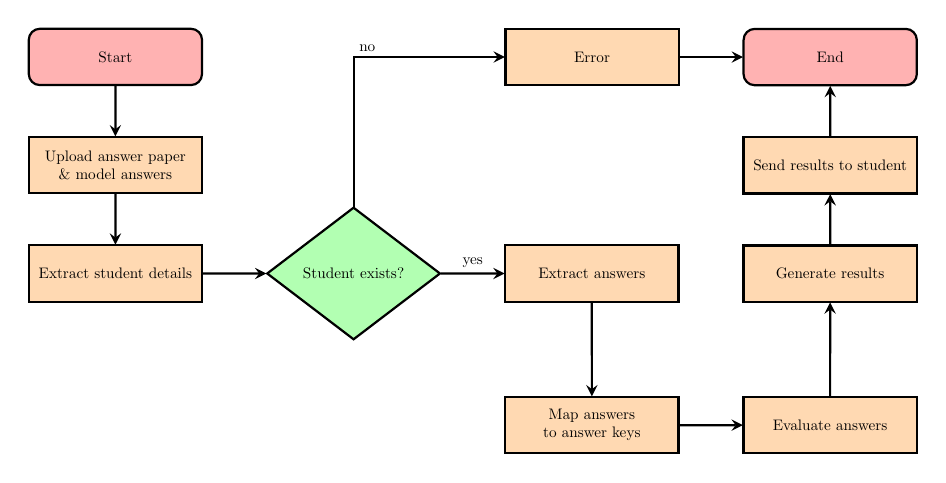
\begin{tikzpicture}[node distance=2.5cm,thick,scale=0.55, every node/.style={scale=0.55}]
            \node (start) [startstop] {Start};
            \node (pro1) [process, below of=start, text width=\textwidth-8.5cm] {Upload answer paper \& model answers};
            \node (pro2) [process, below of=pro1] {Extract student details};
            \node (dec1) [decision, right of=pro2, xshift=3cm] {Student exists?};
            \node (pro3) [process, right of=dec1, xshift=3cm] {Extract answers};
            \node (pro4) [process, text width=\textwidth-8.5cm, below of=pro3, yshift=-1cm] {Map answers to answer keys};
            \node (pro5) [process, right of=pro4, xshift=3cm] {Evaluate answers};
            \node (pro6) [process, above of=pro5, yshift=1cm] {Generate results};
            \node (pro7) [process, above of=pro6] {Send results to student};
            \node (end) [startstop, above of=pro7] {End};
            \node (error) [process, left of=end, xshift=-3cm] {Error};

            \draw [arrow] (start) -- (pro1);
            \draw [arrow] (pro1) -- (pro2);
            \draw [arrow] (pro2) -- (dec1);
            \draw [arrow] (dec1) -- node[anchor=south] {yes} (pro3);
            \draw [arrow] (dec1) |- node[anchor=south west] {no} (error);
            \draw [arrow] (pro3) -- (pro4);
            \draw [arrow] (pro4) -- (pro5);
            \draw [arrow] (pro5) -- (pro6);
            \draw [arrow] (pro6) -- (pro7);
            \draw [arrow] (pro7) -- (end);
            \draw [arrow] (error) -- (end);
        \end{tikzpicture}
        % \caption{}
        % \label{}
    \end{figure}
\end{frame}

\subsection{Data Flow Diagram - Level 0}

\begin{frame}
    \frametitle{Data Flow Diagram - Level 0}
    \begin{figure}[!htb]
        \centering
        \noindent\resizebox{\textwidth}{!}{
            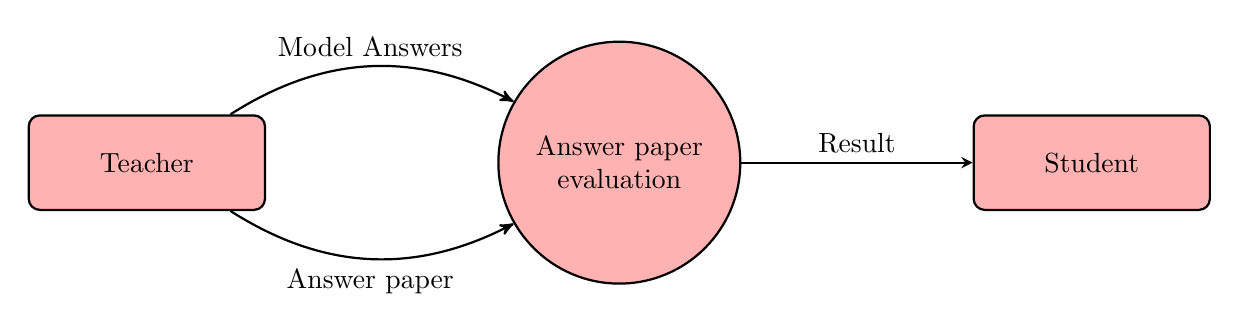
\begin{tikzpicture}[->,>=stealth',auto,node distance=3cm,thick]
                \node (proc1) [dfdprocess] {Answer paper evaluation};
                \node (teacher) [dfdentity, left of=proc1, xshift=-3cm] {Teacher};
                \node (student) [dfdentity, right of=proc1, xshift=3cm] {Student};
    
                % \draw [arrow] (teacher) -- node[anchor=south, text width=3.9cm, text centered] {Answer paper \& Answer key} (proc1);
                \draw [arrow] (proc1) -- node[anchor=south] {Result} (student);
    
                \path
                (teacher) edge[bend right] node [text centered, anchor=north] {Answer paper} (proc1);
                \path
                (teacher) edge[bend left] node [text centered] {Model Answers} (proc1);
            \end{tikzpicture}
        }
        \vspace{0.5cm}
        \caption{Data Flow Diagram Level 0}
        \label{fig:dfd-0}
    \end{figure}
\end{frame}

\subsection{Data Flow Diagram - Level 1}

\begin{frame}
    \frametitle{Data Flow Diagram - Level 1}
    \begin{figure}[!ht]
        % \hspace{-1cm}
        \centering
        \noindent\resizebox{\textwidth}{!}{
            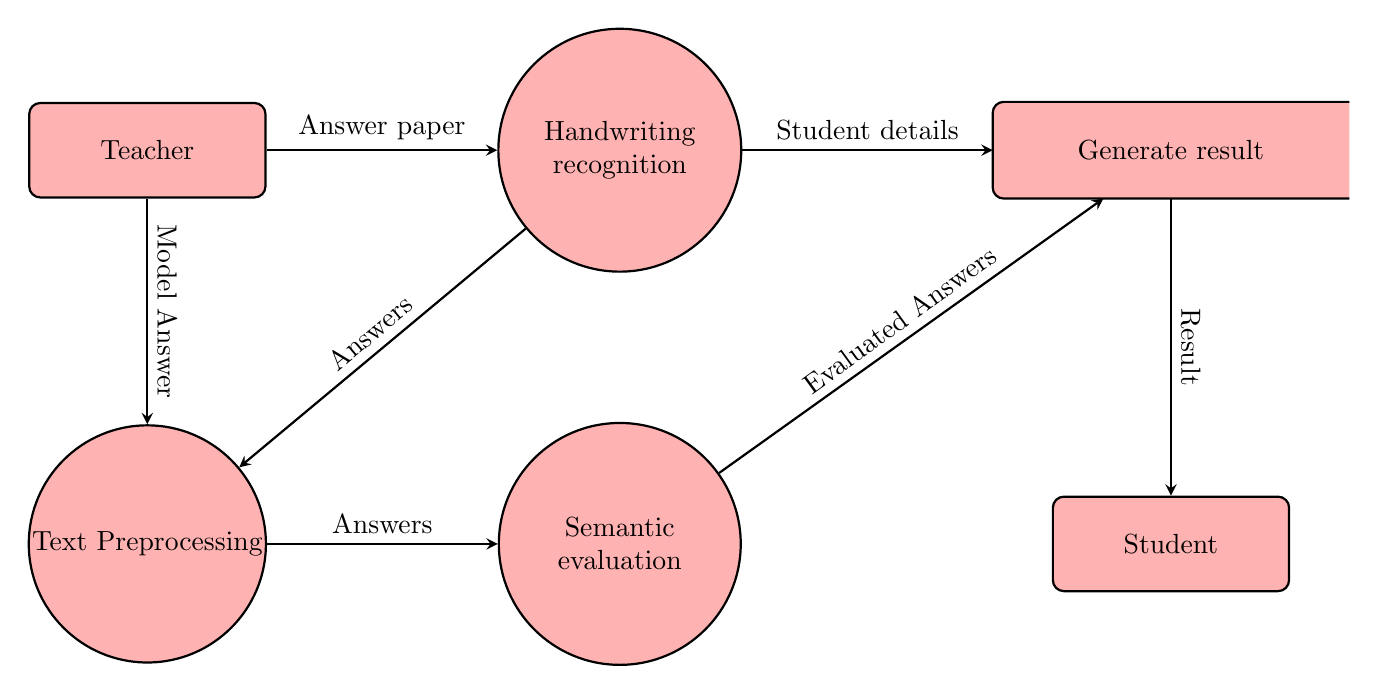
\begin{tikzpicture}[node distance=3cm,thick]
                \node (proc1) [dfdprocess] {Handwriting recognition};
                \node (teacher) [dfdentity, left of=proc1, xshift=-3cm] {Teacher};
                \node (proc2) [dfdprocess, below of=teacher, yshift=-2cm] {Text Preprocessing};
                \node (proc3) [dfdprocess, right of=proc2, xshift=3cm] {Semantic evaluation};
                \node (result) [data store, right of=proc1, xshift=4cm] {Generate result};
                \node (student) [dfdentity, right of=proc3, xshift=4cm] {Student};
    
                \draw [arrow] (teacher) -- node[anchor=south] {Answer paper} (proc1);
                \draw [arrow] (teacher) -- node[rotate=-90, anchor=south] {Model Answer} (proc2);
                \draw[arrow] (proc1) -- node[rotate=40, anchor=south] {Answers} (proc2);
                \draw[arrow] (proc2) -- node[anchor=south] {Answers} (proc3);
                \draw[arrow] (proc3) -- node[rotate=36,anchor=south] {Evaluated Answers} (result);
                \draw[arrow] (result) -- node[rotate=-90, anchor=south] {Result} (student);
                \draw[arrow] (proc1) -- node[anchor=south] {Student details} (result);
            \end{tikzpicture}
        }
        \vspace{0.5cm}
        \caption{Data Flow Diagram Level 1}
        \label{fig:dfd-1}
    \end{figure}
\end{frame}
\section{Conclusion}
\begin{frame}
\frametitle{Conclusion}
\begin{itemize}
    \item We presented a method to recognize handwritten texts using a 
    system based on CNN-LSTM model widely applied to transcribe 
    isolated text lines.
    \item A GUI was provided for teachers and students.
    \item A CER of 8.57\% was obtained.
    \item The WER was relatively high as seen from results.
    \item Semantic analysis was done on a word-word comparison.
    \item This lead to false postives. Need to improve this in the future.
\end{itemize}
\end{frame}


\begin{frame} %allow to expand references to multiple frames (slides)

\frametitle{References}

\scriptsize{\bibliographystyle{plain}}

\bibliography{ref} %bibtex file name without .bib extension
\nocite{*}
\end{frame}

\begin{frame}
\Huge{\centerline{Thank You}}
\end{frame}

\end{document} 